\documentclass[12pt]{article} 

%?? paths
\newcommand{\CiteMathPackage}{../../math} 
\newcommand{\CiteReference}{../reference.bib}

%?? packages 
\usepackage{setspace,geometry,fancyvrb,rotating} 
\usepackage{marginnote,datetime,enumitem} 
\usepackage{titlesec,indentfirst} 
\usepackage{amsmath,amsfonts,amssymb,amsthm,mathtools} 
\usepackage{threeparttable,booktabs,adjustbox} 
\usepackage{graphicx,epstopdf,float,soul,subfig} 
\usepackage[toc,page]{appendix} 
\usdate

%?? page setup 
\geometry{scale=0.8} 
\titleformat{\paragraph}[runin]{\itshape}{}{}{}[.] 
\titlelabel{\thetitle.\;} 
\setlength{\parindent}{10pt} 
\setlength{\parskip}{10pt} 
\usepackage{Alegreya} 
\usepackage[T1]{fontenc}

%?? bibliography 
\usepackage{natbib,fancybox,url,xcolor} 
\definecolor{MyBlue}{rgb}{0,0.2,0.6} 
\definecolor{MyRed}{rgb}{0.4,0,0.1} 
\definecolor{MyGreen}{rgb}{0,0.4,0} 
\definecolor{MyPink}{HTML}{E50379} 
\definecolor{MyOrange}{HTML}{FF5733} 
\definecolor{MyPurple}{HTML}{BF40BF}
\newcommand{\highlightR}[1]{{\emph{\color{MyRed}{#1}}}} 
\newcommand{\highlightB}[1]{{\emph{\color{MyBlue}{#1}}}} 
\newcommand{\highlightP}[1]{{\emph{\color{MyPink}{#1}}}} 
\newcommand{\highlightO}[1]{{\emph{\color{MyOrange}{#1}}}}
\newcommand{\highlightPP}[1]{{\emph{\color{MyPurple}{#1}}}}
\usepackage[bookmarks=true,bookmarksnumbered=true,colorlinks=true,linkcolor=MyBlue,citecolor=MyRed,filecolor=MyBlue,urlcolor=MyGreen]{hyperref} \bibliographystyle{econ}

%?? math and theorem environment 
\theoremstyle{definition} 
\newtheorem{assumption}{Assumption} 
\newtheorem{definition}{Definition} 
\newtheorem{theorem}{Theorem} 
\newtheorem{proposition}{Proposition} 
\newtheorem{lemma}{Lemma} 
\newtheorem{example}{Example} 
\newtheorem{corollary}[theorem]{Corollary} 
\usepackage{mathtools} 
\usepackage{\CiteMathPackage}

\begin{document} 


%??%??%??%??%??%??%??%??%??%??%??%??%??%??%??%??%??%??%??%??%??%?? 
%?? title 
%??%??%??%??%??%??%??%??%??%??%??%??%??%??%??%??%??%??%??%??%??%??

\title{\bf Long-Term Unemployment and the Great Recession: The Role of Composition, Duration Dependence, and Nonparticipation, Journal of Labor Economics, 2016}
\author{Wenzhi Wang \thanks{This note is written in my pre-doc period at the University of Chicago Booth School of Business.} } 
\date{\today}
\maketitle

\citet{kroftLongTermUnemploymentGreat2016}

%??%??%??%??%??%??%??%??%??%??%??%??%??%??%??%??%??%??%??%??%??%?? 
%?? Introduction
%??%??%??%??%??%??%??%??%??%??%??%??%??%??%??%??%??%??%??%??%??%??

\section{Introduction}

This paper investigates whether a search and matching model can explain important features of the US labor market in the Great Recession and its aftermath. In particular, we ask whether such a model can account for the rise in the unemployment rate and the increase in the incidence of long-term unemployment among the unemployed. 

This paper attempts to to account for the two facts documented in Figure \ref{fig2} -- the rise in the long-term unemployment share and the shift in the Beveridge curve -- by exploring the role of \highlightO{shifts in the composition of the unemployed}, \highlightO{duration dependence in job finding rates for the unemployed}, and \highlightO{transitions in and out of the labor force (between unemployment, employment, and nonparticipation)}. To preview our main result, we find that an enriched matching model -- incorporating duration dependence and nonparticipation -- can account for almost all of the increase in the incidence of long-term unemployment and most of the outward shift  in the Beveridge curve during the Great Recession. By contrast, we do not find any evidence that compositional shifts play an important role. 

\setcounter{figure}{1}
\begin{figure}[H]
	\setcounter{subfigure}{0}

	\noindent\caption{Long-term unemployment and the Beveridge Curve.}
	\centering	

	\subfloat[Long-term Unemployment Share in the U.S., 2000-2013]  {\resizebox{0.7\textwidth}{!}{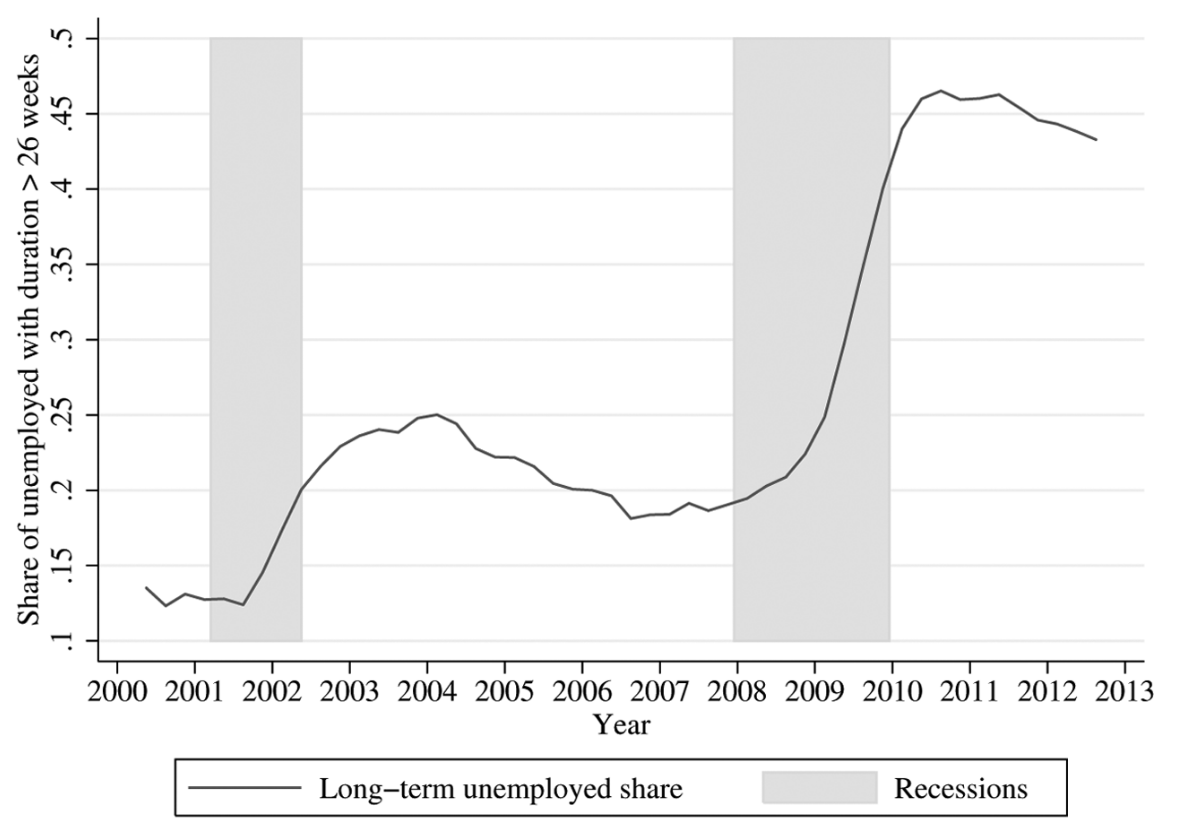
\includegraphics{kroftLongTermUnemploymentGreat2016_fig2A.png}}} \\

	\subfloat [The Beveridge Curve in the U.S., 2000-2013] {\resizebox{0.7\textwidth}{!}{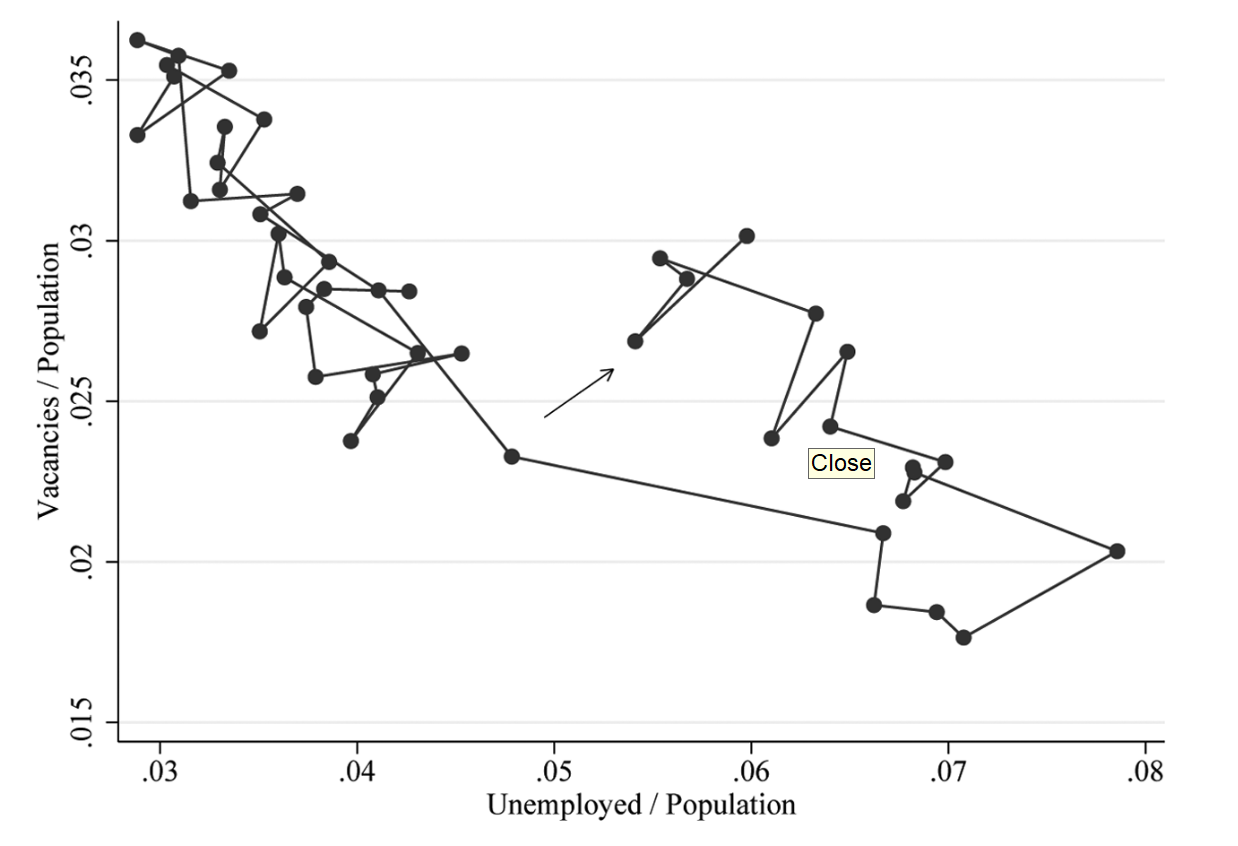
\includegraphics{kroftLongTermUnemploymentGreat2016_fig2B.png}}}

	\label{fig2}
\end{figure}

We begin our analysis by showing that between 2008 and 2013, compositional shifts towards groups with traditionally longer unemployment durations account for very little of the overall rise in the incidence of long-term unemployment documented in Figure \ref{fig2}. We show that long-term unemployment increased for virtually all groups and that compositional shifts do not go very far in accounting for the rise in long-term unemployment. For this exercise, \highlightPP{compositional shifts refer to the changes in observed characteristics of unemployed workers—specifically, variables in the Current Population Survey related to demographics, occupation, industry, region, and the reason for unemployment}. We emphasize that this analysis cannot account for changes in the composition of the unemployed based on unobserved characteristics.

We next examine the extent to which a matching model can account for the observed increase in long-term unemployment and the observed shift in the Beveridge curve. To do this, we enrich a standard matching model along three dimensions. 
\begin{enumerate}[topsep=0pt, leftmargin=20pt, itemsep=0pt, label=(\arabic*)]
	\setlength{\parskip}{10pt} 
	\item First, we allow for duration dependence in the job finding rate of the unemployed.
	\item Second, we allow for flows between employment ($E$), unemployment ($U$), and nonparticipation ($N$), instead of focusing exclusively on flows between $E$ and $U$, as in a standard matching model.
	\item Third, we allow flows from employment and nonparticipation into unemployment to occur not just into short durations but also into long unemployment durations, consistent with observed flows in the CPS. 
\end{enumerate}

We calibrate out enriched matching model using monthly data in the years before the Great Recession (2002-7) and study how well the calibrated model fits the data during the Great Recession, holding fixed the calibrated parameters. In the first step, we measure transition rates between the different labor market states ($E$, $U$, and $N$) over the entire 2002-13 period and estimate duration dependence using data from 2002 to 2007. In the second step, we calibrate the matching model parameters. By first measuring transition rates without imposing the structure of the matching model, we obtain measured hazard rates (between unemployment, employment, and nonparticipation) that are robust to model misspecification. An alternative to our two-step approach would be to estimate the hazard rates and the matching model parameters in a single step. One advantage of our two-step approach is that it clarifies when failures to match the evolution of the job finding rates over this time period are due to shortcomings in the enriched matching model. Another advantage is that it is straightforward to impose alternative assumptions about the magnitude of ``true'' duration dependence to explore the sensitivity of the results (since the second step takes the duration dependence estimates from the first step as given, allowing alternative duration dependence estimates to be ``plugged in'' at the second stage).

In all of our analyses, we treat vacancies, transitions from employment to unemployment and nonparticipation, and transitions between nonparticipation and unemployment as the exogenous ``forcing variables'' of the model. By contrast, we allow the job finding rates (for both the unemployed and nonparticipants), the labor market states, and the distribution of unemployment durations to all evolve endogenously (holding constant the calibrated parameters from the 2002-7 period). Clearly, a more complete model of the economy would endogenize the forcing variables. However, we treat these variables as exogenous because endogenizing them would require a model of vacancy creation as well as a model of labor demand, which is beyond the scope of this paper.

\section{Data}

\section{Long-Term Unemployment and the Great Recession: Assessing the Role of Composition}

%??%??%??%??%??%??%??%??%??%??%??%??%??%??%??%??%??%??%??%??%??%?? 
%?? Matching Framework 
%??%??%??%??%??%??%??%??%??%??%??%??%??%??%??%??%??%??%??%??%??%??

\section{Matching Framework}

In this section, we outline our matching framework, which augments a standard matching model to allow for duration dependence in unemployment and flows to and from nonparticipation. We begin with a standard matching model of the labor market, which models fluctuations in the job finding probability through reduced-form matching function. We enrich this standard matching model to allow for duration dependence in unemployment and we allow a full set of transitions between employment ($E$), unemployment ($U$), and nonparticipation ($N$).

Our goal is to calibrate this model using data from before the Great Recession and assess how well it accounts for outflows from unemployment and nonparticipation into employment between 2008 and 2013. Throughout our analysis, we take the number of vacancies and inflows into unemployment and nonparticipation as given. Theses are the exogenous ``forcing variables'' of the model. The endogenous variables are the full distribution of unemployment durations, the population shares in each labor market state, and the job finding rates of the unemployed and nonparticipants.

Notations:
\begin{enumerate}[topsep=0pt, leftmargin=20pt, itemsep=0pt, label=(\arabic*)]
    \setlength{\parskip}{10pt} 
    \item $P_t$ = population size ($t$ is monthly calendar time) and $\bc{E_t, U_t}$ = number of employed and unemployed individuals with associated rates $\bc{e_t = E_t/P_t, u_t = U_t/P_t}$. Note that the unemployment rate is defined relative to the total population (rather than the labor force), which imposes symmetry with the nonparticipation rate defined below.
    \item $N_t = P_t - E_t - U_t$ = number of nonparticipants. Let the size of the labor force be denoted by $L_t = E_t + U_t$ and the nonparticipation rate by $n_t = N_t/P_t$.
    \item $V_t$ = total number of job vacancies. The number of job vacancies is an exogenous forcing variable during the period 2008-13 in the counterfactual scenarios we describe below.
    \item Flows to unemployment: $\l_t^{\text{EU}}$ (employment $\rightarrow$ unemployment), $\l_t^{\text{NU}}$ (nonparticipation $\rightarrow$ unemployment). Both of these transition rates are forcing variables during the period 2008-13.
    \item Flows to employment: $\l_t^{\text{UE}}$ (unemployment $\rightarrow$ employment), $\l_t^{\text{NE}}$ (nonparticipation $\rightarrow$ employment). These job finding rates are allowed to endogenously evolve during the period 2008-13.
    \item Flows to nonparticipation: $\l_t^{\text{EN}}$ (employment $\rightarrow$ nonparticipation), $\l_t^{\text{UN}}$ (unemployment $\rightarrow$ nonparticipation). Both of these transition rates are forcing variables during the period 2008-13.
\end{enumerate}

\subsection{Labor Market Flows during the Great Recession}

\subsection{Matching Function}

We adapt the standard matching function to allow nonparticipants to find jobs. We assume that nonparticipants and unemployed individuals meet job openings according to the function $$M\of{U + sN, V} = m_0 \bp{U+sN}^\a V^{1-\a}.$$ One may interpret $s$ as the share of the nonparticipants who are ``marginally attached'', or, alternatively, as the search efficiency of nonparticipants relative to the unemployed. 

We assume that the share of meetings with unemployed individuals is given by $U/(U+sN)$, while the remaining share is with nonparticipants. In addition, we assume (for the unemployed) that the probability that a meeting results in a hire depends on the duration of unemployment. In particular, $A\of{d}$ gives the relative hiring probability of an individual with unemployment duration $d$ as compared to a newly unemployed individual (with duration $d$=0). These assumptions imply that the job finding rates for the unemployed and nonparticipants are given, respectively, by the following expressions:
\begin{equation}
    \label{1}
    \l_t^{\text{UE}}\of{x_t; d} = A\of{d} m_0 x_t^{1-\a},
\end{equation}
\begin{equation}
    \label{2}
    \l_t^{\text{NE}}\of{x_t; d} = s m_0 x_t^{1-\a},
\end{equation}
where $x_t = V_t/(U_t + sN_t)$ is a measure of labor market tightness and $d$ is the duration of unemployment. The parametric specification for $\l_t^{\text{UE}}$ assume that there is ``true'' duration dependence in job finding rates out of unemployment, that is, a genuine causal effect of longer unemployment durations on the hazard rate of exit out of unemployment.

We propose a parametric specification for $A\of{d}$ and estimate this function in the pre-Great Recession period, as we describe below. Let the probability density and distribution of ongoing unemployment durations be given by $\t_t\of{d}$ and $\T_t$, respectively. By integrating over the duration distribution, we get the average job finding rate for the unemployed:

\begin{equation}
    \notag
    \l_t^{\text{UE}}\of{x_t} = \int \l_t^{\text{UE}}\of{x_t; \tau} \t_t\of{\tau} d \tau = m_0 x_t^{1-\a} \int A\of{\tau} \t_t\of{\tau} d \tau.
\end{equation}

How does a recession affect the unemployment job finding rate? In a recession, $x_t$ falls, lowering $\l_t^{\text{UE}}\of{x_t; \tau}$, and hence $\l_t^{\text{UE}}\of{x_t}$. The fall in $\l_t^{\text{UE}}\of{x_t}$ affects $\t_t\of{\tau}$, which can feed back into a lower $\l_t^{\text{UE}}\of{x_t}$ through duration dependence and consequently a higher unemployment rate.

Note that 
\begin{equation}
    \notag
    \frac{\l_t^{\text{UE}}}{\l_t^{\text{NE}}} = \frac{\ol{A}_t}{s},
\end{equation}
where $\ol{A}_t = \int A\of{\tau} \t_t\of{\tau} d \tau$. With empirical estimates for $\ol{A}_t$ and the job finding rates, we can solve for $s = \ol{A}_t \bp{\frac{\l_t^{\text{NE}}}{\l_t^{\text{UE}}}}$. The right-hand side varies with $t$, but we assume that $s$ is time invariant, so we can simply take the average of this expression in period 2002-7 to produce an estimate of $s$ to use in our calibrations. Note that we also assume that both $m_0$ and $A\of{d}$ are time invariant: there are no cyclical changes in matching efficiency or cyclical variation in the magnitude of duration dependence.

\subsection{Labor Market Dynamics}

Given the transition rates between employment, unemployment, and nonparticipation, we can express the dynamics of each of these populations as follows.

\begin{equation}
    \label{3}
    \begin{aligned}
        N_{t+1} & = N_t \bp{1 - \l_t^{\text{NU}} - \wh{\l}_t^{\text{NE}}} + E_t \l_t^{\text{EN}} + U_t \l_t^{\text{UN}}, \\
        U_{t+1}\of{0} &= E_t \t_t^{\text{EU}}\of{0} \l_t^{\text{EU}} + N_t \t_t\of{0}\l_t^{\text{NU}}.
    \end{aligned}
\end{equation}

\begin{equation}
    \label{4}
    \begin{aligned}
        U_{t+1}\of{d+1} & = U_t\of{d}\bp{1 - \wh{\l}_t^{\text{UE}}\of{d} - \l_t^{\text{UN}}} + E_t \t_t^{\text{EU}}\of{d} \l_t^{\text{EU}} + N_t \t_t^{\text{NU}}\of{d} \l_t^{\text{NU}}, \\
        E_{t+1} &= P_t - U_{t+1} - N_{t+1}.
    \end{aligned}
\end{equation}


When we construct the counterfactual scenarios, we assume that if nonparticipants move to unemployment, they draw an unemployment duration from the (empirical) distribution of unemployment durations estimated from observed N-to-U transitions (where the empirical distribution is reestimated each quarter for three unemployment categories: $[0, 6)$ months, $[6, 12)$ months, and $\geq 12$ months). Similarly, we also account for the fact that a share of entrants into unemployment from employment report unemployment durations of 6 months or longer, so when employed workers move into unemployment, they draw an unemployment duration from the empirical distribution of unemployment durations (estimated analogously as for nonparticipants above). These two empirical distributions are $\t_t^{\text{NU}}\of{d}$ and $\t_t^{\text{EU}}\of{d}$, respectively. Since this share changes over time and increased during the Great Recession, we estimate these distributions in each year-quarter, and we use this time-varying distribution in our counterfactual simulations.


\bibliography{\CiteReference} 

\end{document}
